Ein homogenes, rechteckiges Brett ist um eine waagrechte, reibungsfreie Achse durch den Punkt D drehbar; D liegt nicht in der Mitte des Bretts. Das Brett wird um \ang{40} gegen die Waagrechte gedreht und in dieser Lage aus der Ruhe losgelassen. Dabei liegt sein Schwerpunkt S genau senkrecht unter D.
\begin{center}
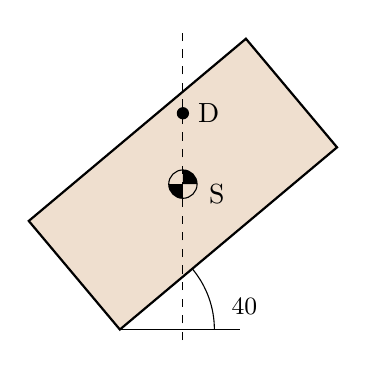
\begin{tikzpicture}[scale=0.6]
 \begin{scope}[rotate=40]
  \fill[brown!25] (-3,-1.5) rectangle (3,1.5);
  \draw[thick] (-3,-1.5) rectangle (3,1.5);
 \end{scope}
 \draw (0,0) circle (0.3); \fill (0,0) -- (0.3,0) arc (0:90:0.3) -- cycle; \fill (0,0) -- (-0.3,0) arc (180:270:0.3) -- cycle;
 \node[right] at (0.35,-0.2) {S};
 \fill (0,1.5) circle (0.13) node[right=2pt] {D};
 \draw[dashed] (0,-3.3) -- (0,3.3);
 \draw (-1.334,-3.077) -- (1.2,-3.077);
 \draw (0.666,-3.077) arc (0:40:2.0);
 \node at (1.3,-2.6) {\small \ang{40}};
\end{tikzpicture}
\end{center}

\begin{abcliste}
\abc
Bleibt das Brett in dieser Lage in Ruhe? Wenn ja: Welche Art von Gleichgewicht ist es?

\abc
Mia meint: „Nein, das Brett ist ja schief. Es dreht sich, bis es waagrecht ist.“ Was ist an ihrer Überlegung falsch?

\abc
Was geschieht, wenn man das Brett aus der gezeichneten Lage ein wenig anstösst?
\end{abcliste}
